%!Tex root = bare_conf.tex

\documentclass[conference]{IEEEtran}
\usepackage{graphicx}
\usepackage{hyperref}
\usepackage[capitalize]{cleveref}
\usepackage{subcaption}

\newcommand{\md} {\textsc{MCTSdvc} }
\newcommand{\cpu} {\textsc{MCTScpu} }
\newcommand{\gpu} {\textsc{MCTSgpu} }


\ifCLASSINFOpdf
\else
\fi

% correct bad hyphenation here
\hyphenation{op-tical net-works semi-conduc-tor}


\begin{document}

\title{Implementing Da Vinci Code Playing Algorithm based on Monte Carlo Tree Search}

% affiliations
\author{
\IEEEauthorblockN{Sangwoo Ji}
\IEEEauthorblockA{Dept. of CSE,
POSTECH\\
Pohang, Republic of Korea\\
sangwooji@postech.ac.kr}
\and
\IEEEauthorblockN{Wonup Jung}
\IEEEauthorblockA{Dept. of CSE,
POSTECH\\
Pohang, Republic of Korea\\
wonup@postech.ac.kr}
\and
\IEEEauthorblockN{Youngjoo Ko}
\IEEEauthorblockA{Dept. of CSE,
POSTECH\\
Pohang, Republic of Korea\\
y0108009@postech.ac.kr}}

\maketitle


% As a general rule, do not put math, special symbols or citations
% in the abstract
\begin{abstract}
%
\end{abstract}

% no keywords



\IEEEpeerreviewmaketitle


\section{Introduction}
% no \IEEEPARstart
 
% Popularity of A.I
Artificial intelligence defeated human play in the game `Go'.
As the number of cases in go is considered much larger than the number of cases in chess or Korean chess, go is treated as the unsolvable game to artificial intelligence.
However, AlphaGo defeated Korean top go player Sedol Lee, and the next version of AlphaGo defeated top go player Ke Jie.
Interestingly, AlphaGo decided to put a stone to a strange location that most go players could not understand~\cite{wierd_alphago}.
Many players shocked about the play of the AlphaGo and tried to learn the new strategies.

% Importance of MCTS
Monte Carlo tree search (MCTS) is a decision making algorithm that is used to implement AlphaGo~\cite{silver2016mastering_alphago}.
MCTS requires large number of simulations, and we hypothesized that large number of simulations led AlphaGo to the strange-but-good location.
The larger number of simulations, the better decision MCTS shows.
However, go has time limit for each turn, the number of simulations for each turn must be limited.

% Success of MCTS. Parallelism
AlphaGo put large number of hardware to increase the number of simulations~\cite{silver2016mastering_alphago}.
The paper-version AlphaGo used 48 CPUs and 8 GPUs.
Those hardware computing unit computes each simulation cases in parallel.
The main factor of defeating human is not only improvement of algorithm, but also improvement of hardware.

% Drawback of MCTS.
However, specific case of the game algorithm can harm the parallelism of MCTS.
GPU-based parallelism exploits the SIMT model that executes the same instruction within many threads.
Therefore, branch instruction harms the parallelism because both of taken branch and non-taken branch need to be executed.
The problem is called \textit{branch divergence}, and high \textit{branch divergence} decreases a program's performance drastically.

% Case study by Da Vinci Code
We found that a board game game 'Da Vinci Code' suffered from branch divergence.
% Not only branch divergence, Da Vinci Code has large number of cases.
The property harm the decision because of two reasons.
Firstly, branch divergence make different length of execution path of each thread, and the shorter-lengthed thread decreased SIMD utilization.
Secondly, branch divergence make large number of MCTS cases, and large number of cases decreased the number of simulations per a case within a fixed time duration.
In Da Vinci Code, each player guess other player's tile.
A player may guess one more tile when the player guessed a tile correctly, and this characteristic makes barnch divergence.
% A player could not know about other player's tile before making a correct dicision, and this randomness makes the number of cases much larger.
We explained the detailed rule of Da Vinci Code~(Section~\ref{sec:davinci}) and interesting features of Da Vinci Code~(Section~\ref{sec:mcts}) later.


% Prove of drawbacks (overhead)
We implement and evaluated two versions of MCTS to compare how branch divergence problem affects decision of MCTS.
We implemented CPU-version of MCTS, called \cpu, which used OpenMP to parallelize simulations.
We implemented GPU-version of MCTS, called \gpu, which used cuda library to parallelize simulations.
% We evaluated \cpu and \gpu to figure out main factor of decreasing performance.
\cpu shown linear fashion performance increasing, whereas \gpu showed non-linear fashion performance increasing and peformance valley.
Performance up to 12 threads increases linearly on \cpu.
Since each core proceeds the thread, performance improvements due to threads increase are limited by the count of cores.

Branch divergence which results from unbalanced game length makes non-linear fashion performance increasing on \gpu
The performance valley result from memory contention as the threads increase. 

We has found the features which makes performance degradation on \gpu which are memory contention, branch divergence.
We will analysis the main feature which causes the performance degradation.
We will optimize \gpu by solving the problems.
We will utilize shared memory and use memory locality to reduce memory contention.
In addition, we will modify the branch statement to reduce branch divergence so that there is not an idle thread left.

% Future plan. Future work. (Discussion)


Intro to rest of the paper

% Monte Carlo Tree Search (MCTS) is a decision making algorithm which has been used for implementing aritifial intelligence(AI) widly.
% Since MCTS is used for games which proceed on real time, it should make decision within a limied time. 
% However, we have to repeat a number of simulated games for good performance of MCTS. 
% If MCTS doesn't have enough simulated games, MCTS can make wrong decision. 
% Therefore parallelism of MCTS not only make right decision, but also reduce the time.\\
% The Da vinci code is the kinds of board game. This game guesses the tiles of opponent based on 

% \hfill mds
 
% \hfill December 23, 2017
\section{Background}

\begin{figure}
\begin{subfigure}[b]{0.95\columnwidth}
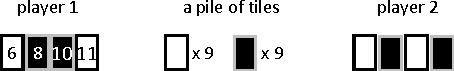
\includegraphics[width=0.95\columnwidth]{figures/DVC_procedure_1.pdf}
\caption{Initial setting}
\label{fig:DVC_procedure_1}
\end{subfigure}
\par\smallskip
\begin{subfigure}[b]{0.95\columnwidth}

\includegraphics[width=0.95\columnwidth]{figures/DVC_procedure_2.pdf}
\caption{Tile selection of palyer 1 (turn 1)}
\label{fig:DVC_procedure_2}
\end{subfigure}
\par\smallskip
\begin{subfigure}[b]{0.95\columnwidth}
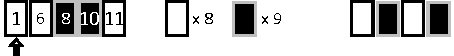
\includegraphics[width=0.95\columnwidth]{figures/DVC_procedure_3.pdf}
\caption{Tile insertion of player 1 (turn 1)}
\label{fig:DVC_procedure_3}
\end{subfigure}
\par\smallskip
\begin{subfigure}[b]{0.95\columnwidth}
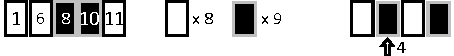
\includegraphics[width=0.95\columnwidth]{figures/DVC_procedure_4.pdf}
\caption{Tile guessing of player 1 (turn 1)}
\label{fig:DVC_procedure_4}
\end{subfigure}
\par\smallskip
\begin{subfigure}[b]{0.95\columnwidth}
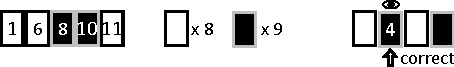
\includegraphics[width=0.95\columnwidth]{figures/DVC_procedure_5.pdf}
\caption{A case that the gussing is correct (turn 1)}
\label{fig:DVC_procedure_5}
\end{subfigure}
\par\smallskip
\begin{subfigure}[b]{0.95\columnwidth}
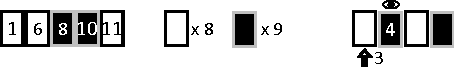
\includegraphics[width=0.95\columnwidth]{figures/DVC_procedure_6.pdf}
\caption{Consecutive tile guessing of player 1 (turn 1)}
\label{fig:DVC_procedure_6}
\end{subfigure}
\par\smallskip
\begin{subfigure}[b]{0.95\columnwidth}
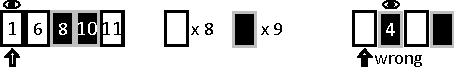
\includegraphics[width=0.95\columnwidth]{figures/DVC_procedure_7.pdf}
\caption{A case that the guessing is wrong (turn 1)}
\label{fig:DVC_procedure_7}
\end{subfigure}
\par\smallskip
\begin{subfigure}[b]{0.95\columnwidth}
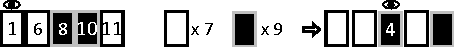
\includegraphics[width=0.95\columnwidth]{figures/DVC_procedure_8.pdf}
\caption{Tile selection of player 2 (turn 2)}
\label{fig:DVC_procedure_8}
\end{subfigure}
\par\smallskip
\begin{subfigure}[b]{0.95\columnwidth}
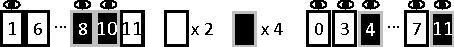
\includegraphics[width=0.95\columnwidth]{figures/DVC_procedure_9.pdf}
\caption{Winning state of player 1 (turn n)}
\label{fig:DVC_procedure_9}
\end{subfigure}
\caption{Procedure of Da Vinci Code}
\end{figure}

\subsection{Da Vinci Code} \label{sec:davinci}

Da Vinci code is a board game that a player guess other player's tiles.
The game use 26 tiles which consists of two joker tiles and numbered tiles from 0 to 11. 
Half of the tiles are black and the others are white, so black 0-11 tiles, a black joker tile, white 0-11 tiles, and a white joker tile exist.
A remaining player wins when other player's all tiles are correctly guessed.

We depicts detailed procedure of Da Vinci Code with an example for clarity.
At first, all the tiles are placed on the table so that all players could not see the tiles' number.
Each player chooses four tiles form the pile and arranges them in ascending order with the smallest number on the left~(\cref{fig:DVC_procedure_1}).
A player could not see other player's tile numbers.
A turn consists of two phases.
Firstly, a player picks up a tile from the pile~(\cref{fig:DVC_procedure_2}) and inserts the tile into the right position~(\cref{fig:DVC_procedure_3}).
Secondly, the player tries to guess the opponent's tiles.
In the example, player 1 guessed the player 2's the first black tile is 4~(\cref{fig:DVC_procedure_4}).
If the tile has the same number, the opponent player must open (reveal) the tile~(\cref{fig:DVC_procedure_5}).
In the case of correct guessing, the player have a chance to guess one more tile.
In the example, we considered that the player decided to guess one more tile~(\cref{fig:DVC_procedure_6}).
When the tile has the different number, the player must open (reveal) the tile the player has brought before~(\cref{fig:DVC_procedure_7}).
When the player decided to stop or made a wrong guess, the next turn is started.
In the next turn, the opponent player conducts the same two phases~(\cref{fig:DVC_procedure_8}).
When the other players' all tiles are opened, the remaining one player wins.
In the example, player 1 wins because all the player 2's tiles are opened~(\cref{fig:DVC_procedure_9}).

\subsection{Monte Carlo Tree Search} \label{sec:mcts}

MCTS is a heuristic search algorithm for making a decision.
% It is mainly used for game play.  
The focus of MCTS is on the analysis of the most successful moves, expanding the search tree based on random sampling of the search space.
The MCTS in games is based on many cases of simulations (or playout).
In each simulation, the game is played out by selecting decision at random.
The final game result of each simulation is used to weight the nodes in the game tree so that better nodes are more likely to be chosen in future simulations.


\begin{figure*}
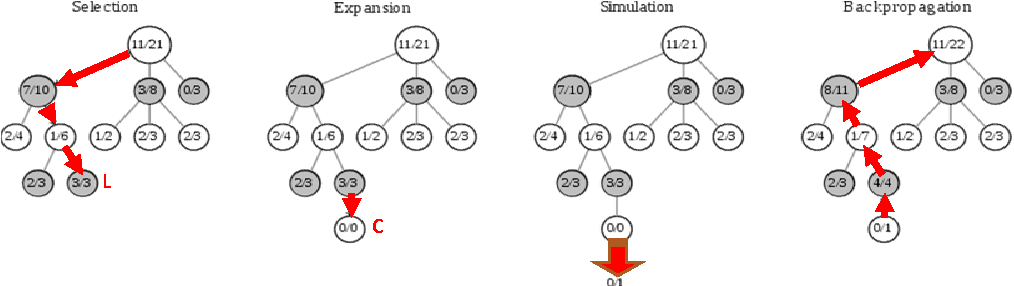
\includegraphics[width=2.05\columnwidth]{figures/MCTS_step.pdf}
\caption{The steps of MCTS}
\label{fig:MCTS_step}
\end{figure*}

There are 4 steps to create MCTS selection expansion, simulation, and backptropagation.
Selection start from root R and select successive child nodes down to a leaf node L. The \cref{fig:MCTS_step} (a) show the selection. shows the selection.
Expansion create one or more child nodes unless leaf node L ends the game and choose node C from one of them. The \cref{fig:MCTS_step} (b) shows the expansion.
Simulation play a random playout from node C as \cref{fig:MCTS_step} (c).
Backpropagation use the result of the playout to update information in the nodes on the path from C to root.
Through these steps, the tree is expanded and used for promising decision.

\section{Motivation}
The MCTS, which is used to make decisions in the game, must complete decisions in a limited amount of time for real-time game play. 
However, in order for MCTS to make good decisions, it is necessary to repeat a number of simulated plays, and when there are not enough simulated plays, a bad answer can be drawn. 
Therefore, parallelization of MCTS is necessary to obtain a high performance answer.
In this project, we will implement the 'DaVinci Code' MCTS to find features that are not suitable for the GPU through comparing GPU based application with CPU based application.
The Da Vinci code has a number of branch divergence and the the time taken to execute command depends on the branch.
In this project, we find the problems which the unsuitable GPU application causes.
We study features that make Da Vinci code-MCTS suitable for GPU compared to CPU based MCTS.

% 일반적으로, implementation은 algorithm 뒤에 오는 경우가 많음.
\section{Method}
We implemented two versions of MCTS for Da Vinci code. 
Firstly, we implemented the MCTS algorithm for Da vinci code (\cpu) that is running upon CPU environment.
We used OpenMP to parallelize the algorithm.
Secondly, we implemented the same algorithm that is running upon GPU environment (\gpu).
We used cuda to implement and parallelize the algorithm.

% Both versions are implemented in parallel. 
In the remaining of this section, we describes each version of algorithm in detail. 
As we modified the algorithm due to compuation overhead, we explain the algorithm design considerations compared to the vanilla version of MCTS.

\subsection{Simplified Algorithm Design}

\begin{figure}
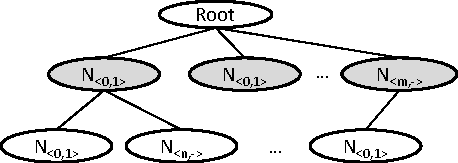
\includegraphics[width=0.95\columnwidth]{figures/base_tree.pdf}
\caption{The base tree of MCTS}
\label{fig:base_tree}
\end{figure}

The \cref{fig:base_tree} shows the overall of MCTS for Da Vinci Code. 
Each node has position and number which are values that a player guesses. Each depth means the game turn. 
We implement simplified algorithm to reduce computation and proceed on real time, since original Da Vinci code has a lot of sibling nodes and child nodes which require a huge amount of computation and time limitation. 
There are two case that we simplified. 
First one is that a player who plays Da Vinci code has two behaviors in each turn, when he/she gussese the tiles. 
Two behaviors are stop and keepping guess. 
If the player guesses correctly, play can select stop or keepping guess. 
Therefore, Original Da Vinci code makes depending on the player's choice. 
However, we implemented Da Vinci code that only stop whether the player hits the tile or not. 
Since original Da vinci code has numerous of child node which make the decision tree unbalanced, we decided to implemente simple Da Vinci code which only has stop behavior.
 
\begin{figure}
\begin{subfigure}[b]{0.95\columnwidth}
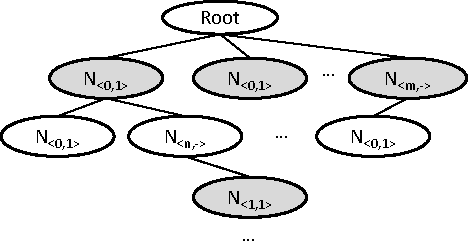
\includegraphics [width=0.95\columnwidth]{figures/sub_compare_expansion_1.pdf}
\caption{Vanilla MCST with expansion}
\label{fig:expansion}
\end{subfigure}
\par\bigskip
\begin{subfigure}[b]{0.95\columnwidth}
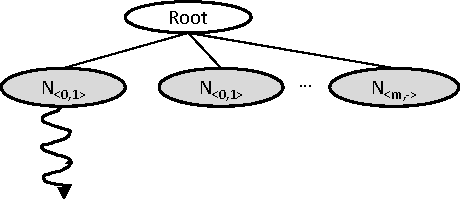
\includegraphics [width=0.95\columnwidth]{figures/sub_compare_expansion_2.pdf}
\caption{Simplified MCST with limited expansion}
\label{fig:limited_expansion}
\end{subfigure}
\caption{Comparr vanilla MCTS with simplified MCTS}
\end{figure}

Second one is original MCTS makes expansion to make decision make tree, but we simplified MCTS. 
Since Da Vinci Code has 000000 on each depth, the number of cases makes a number of sibling nodes too hard to compute decision through MCTS. 
In addition, too many cases make wrong decision, because root node has nodes that have similar winning rate. 
Therefore, MCTS which we implemented has limitation of expansion. 
The \cref{fig:expansion} and \cref{fig:limited_expansion}shows the difference bewteen original MCTS and MCTS which we implemented. 
We make one expansion from root and then the remaining turns are proceeded randomly. 
The result of game updates expanded node from root and the MCTS doesn't make other expansion from frist depth. 


\begin{figure}
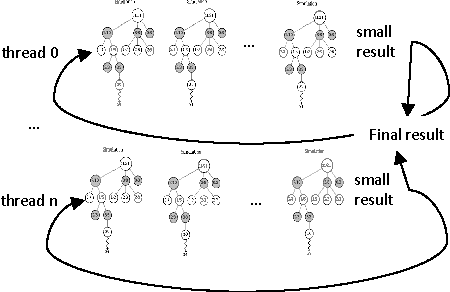
\includegraphics[width=0.95\columnwidth]{figures/implementation.pdf}
\caption{Overall process of creating MCTS}
\label{fig:implementation}
\end{figure}

\subsection{Overall Implementation}
To make final MCTS both of CPU and GPU, each thread make small MCTS by simulating a couple of games.
At this time, MCTS is conducted based on current state of own player and an oppenent.
As playing some games within a thread, a simulation makes small MCTS.
Each game in a thread expands the child node from root. 
When the game expands the child node at the frist turn in a thread, the game proceed randomly. 
The result of game rolls out parent node and is updated on the node which is depth one. 
The next game also expands the child node from the root and update the result of game to expanded node (depth one).
Each tread repeats this routin to make small MCTS. 
The threads have small trees which is from simulation and these trees are combined to final MCTS which is used for decision making in Da Vinci code. 
The \cref{fig:implementation} shows the overall process how the MCTS is conducted.
When the player comes to the turn, threads make final MCTS based on current state of the player and the oppenent. 
The player makes the decision based on the final MCTS. 

\subsection{Implementation of MCTS based on CPU}
MCTS needs many simulated play repeatly to make good decision. 
Parallelism can make MCTS construct good decision tree in a short period due to computating simultaneously. 
MCTS based on CPU is implemented by openMP to utilize parallelism. Each thread computes some turns and derivates a result(win or lose). 
After finish derivation of result, all results from each thread are combined one MCTS.


\subsection{Implementation of MCTS based on GPU}
As we mentioned, MCTS need parallelism to computation many cases for good decision. 
In GPU version, we use CUDA for paraller computation. 
Each tread computes a couple of turns and derivates a result(win or lose) as same as CPU version. 
After finish derivation of result, the results from each tread are combined final MCTS. 


\section{Evaluation}
We implemented MCTS for Da Vincicode upon 4-CPU(Pascal Titan Xp) and 12-core CPU.
We measure the execution time to analysis the dominant factor of time consuming.
We evaluate the performance and difference between CPU based MCTS and GPU based MCTS to measure from the number of simulation per second.

\subsection{Execution Time}
\begin{figure*}
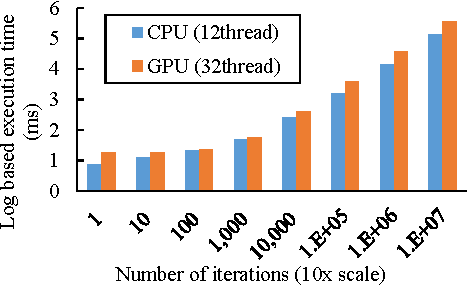
\includegraphics[width=2.05\columnwidth]{figures/time_consuming.pdf}
\caption{The time consuming according to the number of iterations}
\label{fig:time_consuming}
\end{figure*}

We mesure the execution time by varying the number of simulations from 1 to $10^7$ and calculate average values on 5 times execution. 
The \cref{fig:time_consuming} shows the execution time which CPU measures using 12 threads and GPU measures using 32 threads
As increasing the number of simulations, the execution time also increases. Therefore, the number of simulation is dominant factor of time consuming. 

The \cref{fig:time_consuming} shows that the execution is not much different when the number of simulations is small. 
However, as the number of simulations increases, the number of simulations and the execution time are proportional.
The reason is when the number of simulation is small, the memory access to the large array becomes the key factor of the performance. However, when the number of simulation is large, the computing becomes the key factor. Therefore the performance (execution time) is proportional to the number of simulations.

\subsection{The Number of Simulations per Second}
\subsubsection{CPU}
\begin{figure}
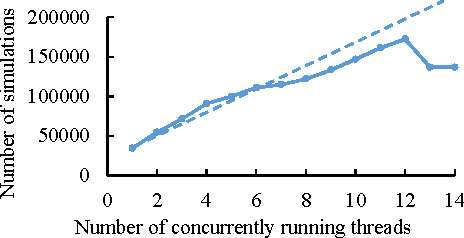
\includegraphics[width=0.95\columnwidth]{figures/cpu_num_simulation.pdf}
\caption{The number of simulations per second on CPU}
\label{fig:cpu_num_simulation}
\end{figure}

The \cref{fig:cpu_num_simulation} shows the result of the number of simulation per second over increasing number of threads of CPU. As incresing threads, the number of simulations per second also increases linearly. 
However, you can see the number of simulations decrease if the number of threads exceeds 12. 
The reason why the number of simulations decrease is that we have only 12 core. In other word, the number of physical cores is the scalability bootleneck. 
Therefore, it can be seen that the performance increases linearly with the number of cores in the CPU. 
\subsubsection{GPU}
\begin{figure}
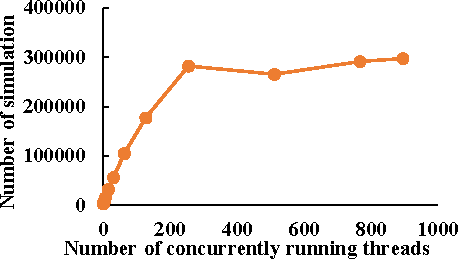
\includegraphics[width=0.95\columnwidth]{figures/gpu_num_simulation.pdf}
\caption{The number of simulations per second on GPU}
\label{fig:gpu_num_simulation}
\end{figure}

The \cref{fig:gpu_num_simulation} shows the result of the number of simulation per second over increasing number of threads of GPU. 
Unlike the \cref{fig:cpu_num_simulation}, the \cref{fig:gpu_num_simulation} shows the non-linear shape. 
In addition, the graph has instant performance degradation at the middle despite increasing the number of threads. 
This is because cache misses increase as the number of thread is used, and memory bottlenecks from cache misses are higher than computaion performance obtained by increasing threads in CPU.

We measure the number of simulations with varying the number of warps to identify the valley which is mentioned in ~\cite{hpca2015valley}. 
\begin{figure}
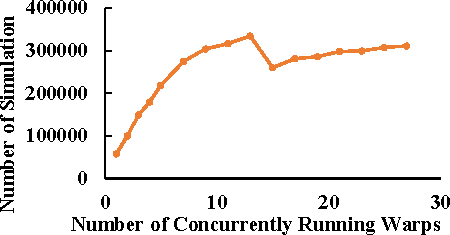
\includegraphics[width=0.95\columnwidth]{figures/gpu_warp_simulation.pdf}
\caption{The number of simulation according to the number of warps on GPU}
\label{fig:gpu_warp_simulation}
\end{figure}

The \cref{fig:gpu_warp_simulation} shows the result of experiment that measures the number of simulations according to the number of warps. 
If the number of warps is over 12, the performance decrease like ~\cite{hpca2015valley}. 
The memory contention makes valley, therefore the the number of simulation reducte despite increasing the number of warps. 

\begin{figure}
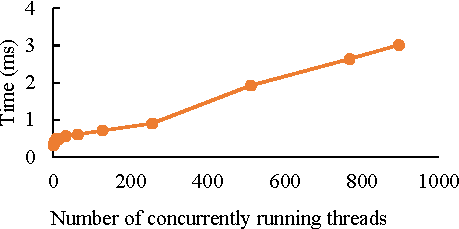
\includegraphics[width=0.95\columnwidth]{figures/gpu_thread_time.pdf}
\caption{How much time takes to execute application on GPU depending on thread size}
\label{fig:gpu_thread_time}
\end{figure}

In MCTS based on GPU, the threads which are already finished should wait until the thread which has the most number of turns ends. 
Because other threads need to wait for the longest thread, the MCTS based on GPU should be the weak scaling which takes the same amount of time to increase the number of threads.
However, the \cref{fig:gpu_thread_time} which shows that weak scaling is not sustained. 
There are two reasons why the \cref{fig:gpu_thread_time} is not weak scaling. 
First is path divergence issue until 16 threads. 
Many divergences to guess the opponent's tile take more time to finish compuation.   
Second is memory contention issue which performance valley as we mentioned previous more than 16 threads.
As the number of threads increases, not enough memory makes memory contention so the time takes more time.


\section{Discussion}
\subsection{Parallelization in GPU and CPU}
To make good MCTS, parallelization can help simulate a number of cases in limited time. 
However, paralleization makes bottleneck in two versions of MCTS for Da vinci code.
For \cpu, the number of physical cores becomes a bottleneck of performance improvement.
For \gpu, memory contention and path divergence interfere performance improvement. 
In order to utilize parallelization well, MCST should be optimized for Da Vinci code to solve the bottleneck.

\subsection{Challenges during the project} %Davinci code가 MCTS에 맞지 않아서 구현이 힘들었다
We implemented \cpu and \gpu to compare performance of MCTS for Da Vinci code. 
However Da Vinci code is not suitable for the structure of MCTS because of unbalanced length of turn and a lot of cases.
Huge cases makes numerous sibling nodes so it is hard to conduct MCTS. 
In addition unbalanced lenth causes path divergence so it is hard to parallize.
This structural problem has made it difficult to implement the MCTS.

\subsection{Future works}
To optimize the MCTS, we need to analysis the main factor of memory contention with controlling memory consumption per thread. 
Through identifing the cause of bottleneck, we need to design the MCTS to solve this problem.
\section{Conclusion}
We implement \cpu and \gpu for Da Vinci code for parallelization. 
To Compare \cpu with \gpu, we measure the execution time with increasing the number of simulation and the number of simulation with increasing thread. 
Through the result, \cpu show well strongly scaled in parallelization while \gpu show non-weakly scaled due to memory contention. 




% conference papers do not normally have an appendix


% use section* for acknowledgment
\section*{Acknowledgment}


The authors would like to thank...





% trigger a \newpage just before the given reference
% number - used to balance the columns on the last page
% adjust value as needed - may need to be readjusted if
% the document is modified later
%\IEEEtriggeratref{8}
% The "triggered" command can be changed if desired:
%\IEEEtriggercmd{\enlargethispage{-5in}}

% references section

% can use a bibliography generated by BibTeX as a .bbl file
% BibTeX documentation can be easily obtained at:
% http://mirror.ctan.org/biblio/bibtex/contrib/doc/
% The IEEEtran BibTeX style support page is at:
% http://www.michaelshell.org/tex/ieeetran/bibtex/
%\bibliographystyle{IEEEtran}
% argument is your BibTeX string definitions and bibliography database(s)
%\bibliography{IEEEabrv,../bib/paper}
%
% <OR> manually copy in the resultant .bbl file
% set second argument of \begin to the number of references
% (used to reserve space for the reference number labels box)

% \begin{thebibliography}
\bibliographystyle{IEEEtran}
\bibliography{reference}
% \end{thebibliography}




% that's all folks
\end{document}


